\documentclass[12pt]{article}
\usepackage{amsmath}
\usepackage{hyperref}
\usepackage{listings}
\usepackage{xcolor}
\usepackage{graphicx}

\lstset{
  language=C++,
  basicstyle=\ttfamily,
  keywordstyle=\color{blue},
  commentstyle=\color{gray},
  stringstyle=\color{red},
  numbers=left,
  numberstyle=\tiny\color{gray},
  stepnumber=1,
  numbersep=5pt,
  backgroundcolor=\color{lightgray!20},
  tabsize=2,
  showspaces=false,
  showstringspaces=false,
  breaklines=true
}
\title{\LARGE C++ Variable Types}
\author{\LARGE Nisa Çontay}
\date{\today}

\begin{document}

\maketitle

\newpage


\section{Introduction}
C++ programming language has various data types. These types are primarily divided into two main categories: integer types and floating-point types. In this report, we will examine the fundamental and extended data types in C++ as well as fixed-width data types.
\section{Integer}

\subsection{Basic Integer Types}
\begin{itemize}
    \item \texttt{int}: Standard integer type. Its size is usually 4 bytes. Meaning, it can store values from -2147483648 to 2147483647.
    \item \texttt{short int} or \texttt{short}: Small-sized integer type. Its size is usually 2 bytes. It's range is -32768 to 32767.
    \item \texttt{long int} or \texttt{long}: Large-sized integer type. It's size is at least 4 bytes. The exact size of long can vary depending on the platform and compiler. On some platforms, long might be 64 bits, while on others, it remains 32 bits.
    \item \texttt{long long int} or \texttt{long long}: Even larger-sized integer type. It stores at least 8 bytes.long long provides a more consistent size across different platforms, typically being 64 bits.
\end{itemize}

\subsection{Signed and Unsigned Integer Types}
\begin{itemize}
    \item \texttt{unsigned int} veya \texttt{unsigned}: Unsigned int can only represent non-negative integer values. A 32-bit unsigned integer can store only positive values from 0 to 4294967295. Wraps around to 0 if the value exceeds the maximum limit.
    \item \texttt{signed int} veya \texttt{signed}: Signed int can represent both positive and negative values. A signed integer can hold values from -2147483648 to 2147483647. A signed integer can get an overflow error while used in a program with larger values.
\end{itemize}
\subsection{Fixed Width Integer Types}
\begin{itemize}
    \item\texttt{int8\_t}, \texttt{int16\_t}, \texttt{int32\_t}, \texttt{int64\_t}: Signed integer type with width of
exactly 8, 16, 32 and 64 bits respectively
with no padding bits and using 2's complement for negative values
(provided only if the implementation directly supports the type)
    \item\texttt{int\_fast8\_t}, \texttt{int\_fast16\_t}, \texttt{int\_fast32\_t}, \texttt{int\_fast64\_t}: Fastest signed integer type with width of at least 8, 16, 32 and 64 bits respectively. Used when performance is more critical than the exact size. This type allows the compiler to select the most efficient integer type that meets the minimum size requirement. When we use this type, we only specify the minimum size we need, and then the compiler selects the most efficient version. It can be the exact size we chose or it can be bigger.
    \item\texttt{int\_least8\_t}, \texttt{int\_least16\_t}, \texttt{int\_least32\_t}, \texttt{int\_least64\_t}: Smallest signed integer type with width of at least 8, 16, 32 and 64 bits respectively. Used when minimizing memory usage is more critical than performance. This type ensures the smallest type that meets the minimum size requirement.
    \item\texttt{intmax\_t}: maximum width integer type.
    \item\texttt{intptr\_t}: integer type capable of holding a pointer.
    \item\texttt{uint8\_t}, \texttt{uint16\_t}, \texttt{uint32\_t}, \texttt{uint64\_t}: unsigned integer type with width of
exactly 8, 16, 32 and 64 bits respectively
(provided only if the implementation directly supports the type)
    \item\texttt{uint\_fast8\_t}, \texttt{uint\_fast16\_t}, \texttt{uint\_fast32\_t}, \texttt{uint\_fast64\_t}: fastest unsigned integer type with width of
at least 8, 16, 32 and 64 bits respectively
    \item\texttt{uint\_least8\_t}, \texttt{uint\_least16\_t}, \texttt{uint\_least32\_t}, \texttt{uint\_least64\_t}:smallest unsigned integer type with width of
at least 8, 16, 32 and 64 bits respectively
    \item\texttt{uintmax\_t}: maximum width unsigned integer type.
    \item\texttt{uintptr\_t}: unsigned integer type capable of holding a pointer.
\end{itemize} 
\section{Float}
\subsection{Basic Float Types}
\begin{itemize}
    \item \texttt{float}: Single-precision floating-point numbers, typically occupying 32 bits and providing approximately 7 decimal digits of precision.
    \item \texttt{double}: Double-precision floating-point numbers, typically occupying 64 bits and providing approximately 15-16 decimal digits of precision, offering greater precision than float.
    \item \texttt{long double}: Extended-precision floating-point numbers, typically occupying more than 64 bits (usually 80 bits on most platforms) and providing even higher precision than double, often used for specialized numerical computations requiring extremely high precision.
\end{itemize}
\subsection{Fixed Width Float Types}
    According to cppreference, fixed width floating-point types are available since C++23. With <stdfloat> library, it offers to use "float8\_t, float16\_t, float32\_t, float864\_t". Here is an example for it's use:
    \begin{lstlisting}
#include <stdfloat>
#if __STDCPP_FLOAT64_T__ != 1
    #error "64-bit float type required"
#endif
int main()
{
    std::float64_t f = 0.1f64;
}
    \end{lstlisting}
\section{Character}
\subsection{Character Types}
\begin{itemize}
    \item \texttt{char}:Fundamental data type used to represent a single character, typically occupying 1 byte of memory.
    \item \texttt{unsigned char}:Fundamental data type that represents a single byte, capable of storing values from 0 to 255. It is often used for raw binary data manipulation or when working with byte-oriented data that should not have negative values.
    \item \texttt{signed char}:Fundamental data type that represents a single byte, capable of storing values from -128 to 127. It is explicitly used when the signedness of the char type needs to be specified, ensuring that the stored values can include negative numbers.
    \item \texttt{wchar\_t}:Fundamental data type used to represent wide characters, which allows for the storage of a larger set of characters than the standard char type. Typically, wchar\_t is used for handling Unicode or other extended character sets, and its size is platform-dependent, often being 2 or 4 bytes. This type is useful for internationalization and working with non-ASCII text.
    \item \texttt{char8\_t}:Data type introduced in C++20 to represent UTF-8 encoded characters.
    \item \texttt{char16\_t}:Data type introduced in C++20 to represent UTF-16 encoded characters.
    \item \texttt{char32\_t}:Data type introduced in C++20 to represent UTF-32 encoded characters.
\end{itemize}
\section{Boolean}
In C++, `bool` is a fundamental data type representing boolean values, which can be either `true` or `false`. It is commonly used for decision-making in control flow statements like `if`, `while`, and `for`. `bool` variables can be initialized with the keywords `true` or `false` or the result of comparison or logical operations. They occupy 1 byte of memory, although only 1 bit is necessary to store the value. 
\newpage
\section{Some Important Keywords}
\begin{itemize}
    \item \texttt{auto}:The auto keyword in C++ is used to declare variable types automatically. It simplifies code by eliminating the need to explicitly specify the type, especially for complex or lengthy types. However, it can reduce the readability and precision of code and may lead to ambiguity, such as whether a variable is float or double.(since C++11)
    \begin{lstlisting}
#include <iostream>
int main() {
auto num = 1.0; // float or double?
auto name = xyz; // string
}
    \end{lstlisting}
    
    \item \texttt{const}:The const keyword is used to define constants, which are variables whose values cannot be modified after initialization. It can be applied to various types of data, including variables, pointers, and member functions, to ensure their immutability. If we try to change const variable, error occurs.
    
    \begin{lstlisting}
#include <iostream>
class MyClass {
public:
    MyClass(int val) : value(val) {}
    int getValue() const {
        return value;
    }
    void setValue(int val) {
        value = val;
    }
private:
    int value;
};
int main() {
    const int maxValue = 100;
    std::cout << "Max Value: " << maxValue << std::endl;
    int x = 10;
    const int* ptrToConst = &x;
    int* const constPtr = &x;
    const int* const constPtrToConst = &x;
    MyClass obj(10);
    std::cout << "Initial Value: " << obj.getValue() << std::endl;
    obj.setValue(20);
    std::cout << "Updated Value: " << obj.getValue() << std::endl;
    return 0;
}
    \end{lstlisting}
    \item \texttt{constexpr}: Constexpr can be used for objects, functions and constructors and it is evaluated at compile time or at runtime and can represent constants.If a constexpr function is called with constant expressions as arguments, the call can be evaluated at compile time. If called with non-constant expressions, the call is evaluated at runtime.(since C++11)
    \begin{lstlisting}
#include <iostream>
constexpr int square(int x) {
    return x * x;
}
int main() {
    constexpr int result1 = square(5); // Evaluated at compile time
    int y = 6;
    int result2 = square(y); // Evaluated at runtime
}
    \end{lstlisting}
    \item \texttt{consteval}: It is used to indicate that a function must be evaluated at compile time. This means the function is required to produce a constant expression, and it cannot be used in a context where it would be evaluated at runtime. Any call to a consteval function with arguments that are not constant expressions will result in a compile-time error.Ensures that certain computations are guaranteed to be done at compile time, enhancing performance and enabling more robust compile-time checks.(since C++20)
    \begin{lstlisting}
#include <iostream>
consteval int factorial(int n) {
    return (n <= 1) ? 1 : (n * factorial(n - 1));
}
int main() {
    constexpr int fact5 = factorial(5); // Valid: Evaluated at compile time
    int num = 6;
    // int fact6 = factorial(num); // Error: num is not a constant expression
}

    \end{lstlisting}
    \item \texttt{constinit}: It is used to ensure that a variable with static or thread storage duration is initialized at compile time. This can help prevent issues related to the order of initialization of static variables, a common source of bugs in C++. Using constinit can be particularly useful in large projects where the initialization order of static variables in different translation units is complex and critical to the program's correctness. (since C++20)
    \begin{lstlisting}
// consteval function evaluated at compile time
consteval int compute() {
    return 42;
}
// Initialize a global variable at compile time with constinit
constinit int global_value = compute();
void example() {
    // Initialize a static variable at compile time with constinit
    static constinit int static_value = compute();

    // Initialize a thread-local variable at compile time with constinit
    thread_local constinit int thread_value = compute();
}
int main() {
    std::cout << "Global value: " << global_value << std::endl;
    example();
    // Static and thread_local variables can be used within the function where they are defined
    std::cout << "Static value: " << static_value << std::endl;
    std::cout << "Thread-local value: " << thread_value << std::endl;
    return 0;
}
    \end{lstlisting}
    \item \texttt{mutable}: The mutable keyword in C++ allows a member of an object to be modified even if the object itself is const. This is useful when you need to change the state of a member that doesn't logically change the object's observable state. Essentially, it allows certain members of a class to be exempt from the const restrictions.
    \begin{lstlisting}
#include <iostream>
class Counter {
public:
    void increment() const {
        ++count;
    }
    int getCount() const {
        return count;
    }
private:
    mutable int count = 0;  // mutable allows modification even in const functions
};
int main() {
    const Counter counter;  // Create a const object of Counter
    counter.increment();  // Allowed because increment() is a const function but modifies a mutable member
    std::cout << "Count: " << counter.getCount() << std::endl;  // Output: Count: 1
    return 0;
}
    \end{lstlisting}
    \item \texttt{volatile}: It is used to indicate that a variable's value may be changed by something outside the control of the program, such as hardware or a different thread. This keyword is a type qualifier that prevents the compiler from optimizing code involving the volatile variable, ensuring that every access to the variable is actually performed and not optimized away.
    \begin{lstlisting}
#include <iostream>
volatile bool stopFlag = false;  // This variable can be changed externally
void checkFlag() {
    std::cout << "Waiting for stopFlag to become true...\n";
    while (!stopFlag) {
        // Do nothing, just wait
    }
    std::cout << "stopFlag is now true, exiting loop.\n";
}
int main() {
    // Simulate an external change to stopFlag
    std::this_thread::sleep_for(std::chrono::seconds(1));  // Wait for 1 second
    stopFlag = true;  // Change the flag value
    checkFlag();  // Call the function that waits for the flag to change
    return 0;
}
    \end{lstlisting}
    \item \texttt{decltype}: In C++, decltype is a keyword that inspects the declared type of an expression. It was introduced in C++11 and is useful for writing generic code and templates where you might need to deduce the type of a variable or expression without explicitly specifying it.
    \begin{lstlisting}
#include <iostream>

int main() {
    int x = 5;
    decltype(x) y = 10;  // y is deduced to be of type int, same as x

    std::cout << "x: " << x << ", y: " << y << std::endl;
    return 0;
}
    \end{lstlisting}
    \item \texttt{final}: In C++, the final keyword is used to prevent further inheritance of a class or to prevent overriding a virtual function in derived classes. This keyword was introduced in C++11 to enhance the control over the inheritance and polymorphism mechanisms in object-oriented programming.
    \begin{lstlisting}
class Base {
public:
    virtual void show() {
        std::cout << "Base class show function" << std::endl;
    }
};
class Derived final : public Base {
public:
    void show() override {
        std::cout << "Derived class show function" << std::endl;
    }
};
// This will cause a compile-time error because Derived is final
// class AnotherDerived : public Derived {
// };
int main() {
    Derived d;
    d.show();
    return 0;
}
    \end{lstlisting}
\end{itemize}
\section{Terminal Outputs}
\begin{figure}[h]
    \centering
    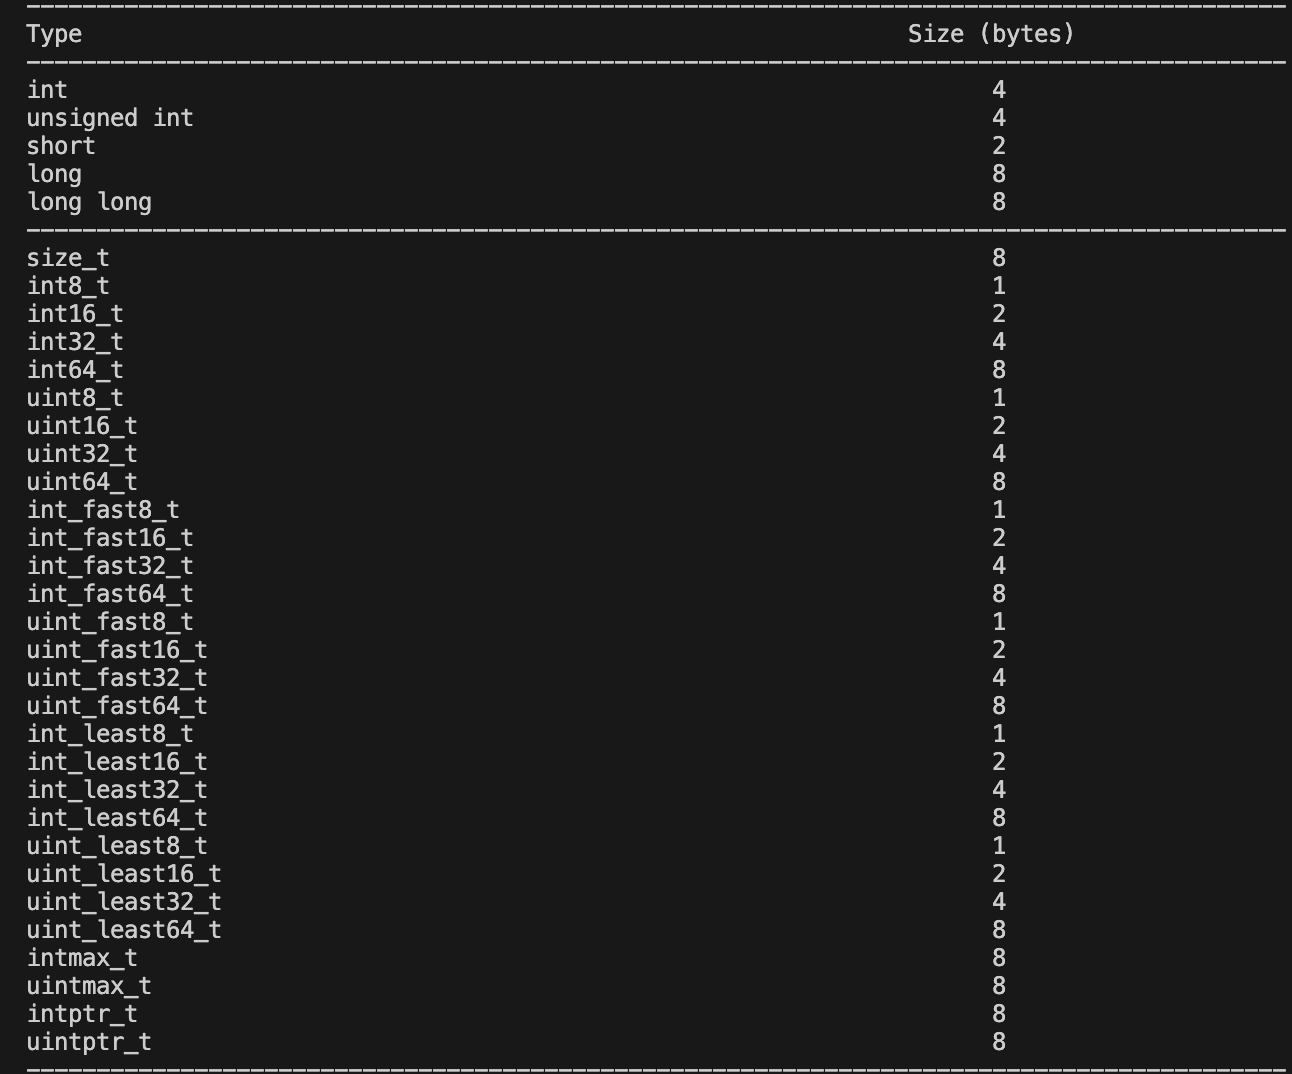
\includegraphics[width=1\textwidth]{intByte.png} 
    \caption{Integer Bytes}
    \label{fig:example-image}
\end{figure}
\begin{figure}[h]
    \centering
    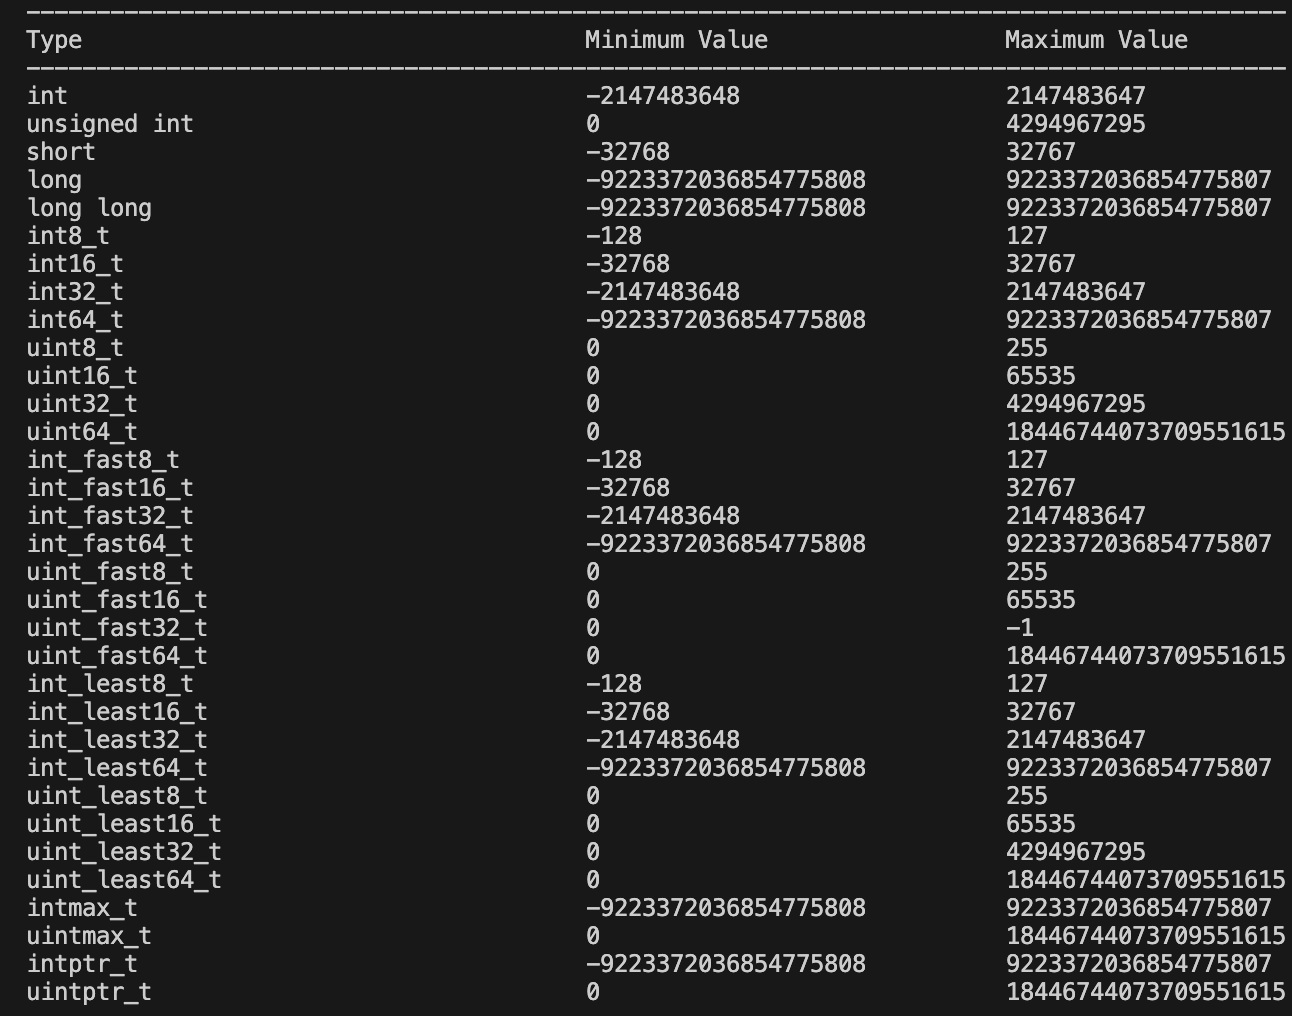
\includegraphics[width=1\textwidth]{intMinMax.png} 
    \caption{Integer Minimum and Maximum Values}
    \label{fig:example-image}
\end{figure}
\begin{figure}[h]
    \centering
    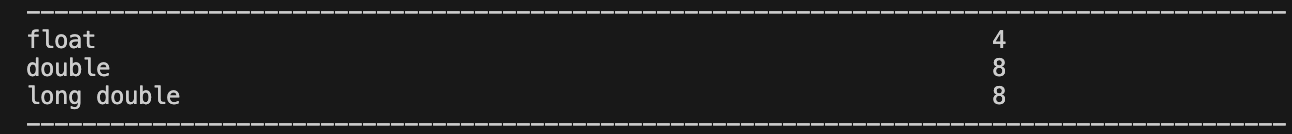
\includegraphics[width=1\textwidth]{floatByte.png} 
    \caption{Float Bytes}
    \label{fig:example-image}
\end{figure}
\begin{figure}[h]
    \centering
    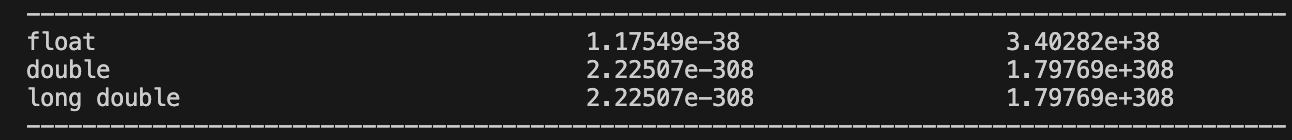
\includegraphics[width=1\textwidth]{floatMinMax.png} 
    \caption{Float Minimum and Maximum Values}
    \label{fig:example-image}
\end{figure}
\begin{figure}[h]
    \centering
    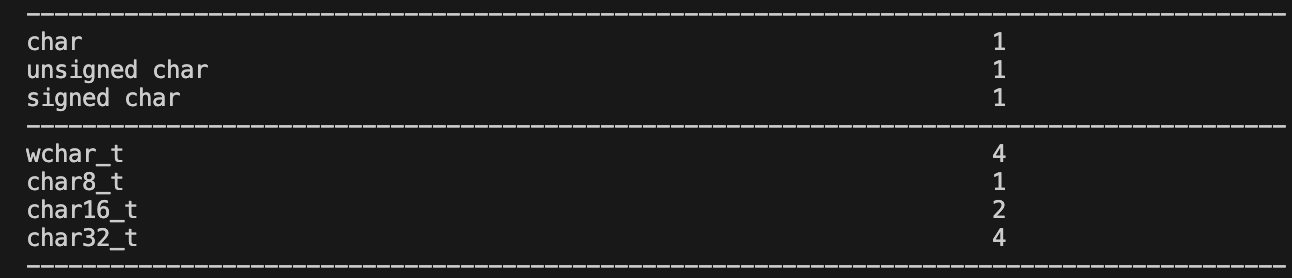
\includegraphics[width=1\textwidth]{charByte.png} 
    \caption{Char Bytes}
    \label{fig:example-image}
\end{figure}
\begin{figure}[h]
    \centering
    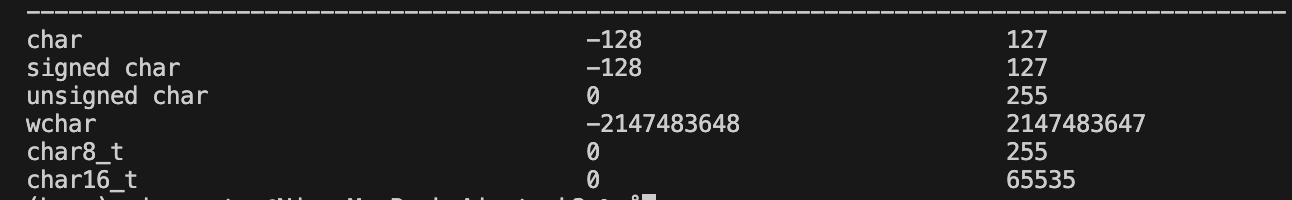
\includegraphics[width=1\textwidth]{charMinMax.png} 
    \caption{Char Minimum and Maximum Values}
    \label{fig:example-image}
\end{figure}
\end{document}
